%!LW recipe=pdfLaTeXmk
\documentclass[scheme=plain,aspectratio=169]{beamer}
\usepackage[T1]{fontenc}
\usepackage{fontawesome5}
\usepackage{mathtools}
\usepackage{tikz}
\usepackage{booktabs}
\usepackage{caption}
\usepackage{outlines}
\usepackage{graphicx}
\usepackage{float}
\usepackage{amsthm}
\usepackage{tabularray}
\usepackage{minted}
\usepackage{hyperref}
\usepackage{cleveref}
\usepackage{url}
\usepackage{xspace}
\usepackage{academicons}
\usepackage{pgfplots}
\usepackage{pgfgantt}
\usepackage{qrcode}
\usepackage{ninecolors}
\usepackage{soul}
\usepackage{tgheros}
\usepackage{xparse}
\usepackage[
  citestyle=authoryear,
  bibstyle=authoryear,
  backend=biber,
  url=false,doi=false,isbn=false
]{biblatex}
\newmintinline[code]{html}{fontsize=\small}
\addbibresource{yuxuan.bib}
\addbibresource{custom.bib}
\DeclareCiteCommand{\silentfootcitetext}
  {\usebibmacro{prenote}}
  {\printtext[bibhyperref]{%
     \printnames{labelname}%
     \addcomma\space
     \usebibmacro{cite:labeldate+extradate}%
     \iffieldundef{booktitle}
       {\iffieldundef{journaltitle}
          {\iffieldundef{eprint}
             {}
             {\addcomma\space
              \iffieldundef{archiveprefix}
                {\printfield{eprint}}
                {\printfield{archiveprefix}\addcolon\printfield{eprint}}}}
          {\addcomma\space\printfield{journaltitle}}}
       {\addcomma\space\printfield{booktitle}}}}
  {\multicitedelim}
  {\usebibmacro{postnote}}
\newcommand{\silentfootcite}[1]{%
  {%
    \setbeamertemplate{footnote}{%
      \parindent 0em\noindent\raggedright\insertfootnotetext\par%
    }%
    \footnotetext{\silentfootcitetext{#1}}%
  }%
}
\newcommand{\todo}[1]{\sethlcolor{red!30!white}\hl{#1}}

\usetheme[
    progressbar=frametitle,
    numbering=fraction,
    subsectionpage=progressbar,
    titleformat title=smallcaps,
    titleformat subtitle=smallcaps,
    titleformat section=smallcaps,
    titleformat frame=smallcaps]{moloch}

\setbeamercolor{palette primary}{bg=gray1}
\setbeamercolor{frametitle}{bg=black,fg=white}
\setbeamercolor{progress bar}{fg=black}
\setbeamerfont{footnote}{size=\tiny}
\renewcommand{\cite}{\footcite}

\definecolor{ForestGreen}{RGB}{34,139,34}
\definecolor{barpos}{HTML}{2F6E73}
\definecolor{barneg}{HTML}{C0392B}
\definecolor{whisk}{HTML}{B5B5B5}
\definecolor{zeroln}{HTML}{CBCBCB}
\definecolor{tickgray}{HTML}{9A9A9A}
% helper for the Post-Study Ratings diverging Likert bars (must live in preamble, not in-frame)
\newcommand{\likertbar}[5]{%
  \draw[whisk,line width=1pt] ({#2-#3},#1) -- ({#2+#3},#1);
  \draw[whisk,line width=1pt] ({#2-#3},#1-0.12) -- ({#2-#3},#1+0.12);
  \draw[whisk,line width=1pt] ({#2+#3},#1-0.12) -- ({#2+#3},#1+0.12);
  \draw[#4,line width=10pt,line cap=round] (0,#1) -- (#2,#1);
  \node[#4,anchor=west,font=\small\bfseries] at ({#2+#3+0.12},#1) {#5};
}
\newcommand{\highlightRelevantValue}[1]{%
  \ifdim #1pt > 0pt
    {\color{ForestGreen}{#1\%}}%
  \else
    {\color{red}{#1\%}}%
  \fi
}


\NewDocumentCommand{\imageframe}{m O{1}}{
  \begin{frame}[plain]
    \begin{tikzpicture}[remember picture,overlay]
      \node[anchor=center, inner sep=0] at (current page.center) {
        \includegraphics[
          width=#2\paperwidth,
          height=#2\paperheight,
          keepaspectratio
        ]{#1}
      };
    \end{tikzpicture}
  \end{frame}
}

\usetikzlibrary{calc}
\setcounter{tocdepth}{1}

\makeatletter
\newlength{\frametitle@padding}
\setlength{\frametitle@padding}{2.2ex}
\newcommand{\frametitlestrut@start}{
  \rule{0pt}{\frametitle@padding +%
    \totalheightof{%
      \ifcsdef{frametitleformat}{\frametitleformat X}{X}%
    }%
  }%
}

\newcommand{\frametitlestrut@end}{
  \rule[-\frametitle@padding]{0pt}{\frametitle@padding}
}

\setbeamertemplate{frametitle}{
    \nointerlineskip%
    \begin{beamercolorbox}[%
        wd=\paperwidth,%
        sep=0pt,%
        leftskip=\frametitle@padding,%
        rightskip=\frametitle@padding,%
      ]{frametitle}%
    \frametitlestrut@start%
    \insertframetitle%
    \hfill%
    \nolinebreak%
    \frametitlestrut@end%
    \end{beamercolorbox}%
    \begin{tikzpicture}[remember picture,overlay]
        \coordinate (logo) at ([xshift=-1.8cm,yshift=-0.5cm]current page.north east);
        \node at (logo) {
\includegraphics[height=.1\textheight]{figures/webserv/northeastern.eps}};
    \end{tikzpicture}
}
\makeatother

\setbeamertemplate{footline}{
    \hbox{
    \begin{beamercolorbox}[wd=\paperwidth,ht=3ex,dp=1.5ex,leftskip=2ex,rightskip=2ex]{page footer}%
        \usebeamerfont{title in head/foot}%
        \hfill
        \begin{tblr}{
            width=.8\linewidth,
            colspec={X[5,l]X[r]}
        }
            \insertsectionhead{}
            % &
            % \ifx\insertsubsection\empty
            % \else
            % \insertsubsection{} 
            % \fi
            &
            \insertframenumber{} / \inserttotalframenumber
        \end{tblr}
        \hfill{}
    \end{beamercolorbox}}%
}


\defbeamertemplate{section page}{my progressbar}{
  \centering
  \begin{beamercolorbox}[wd=\paperwidth,leftskip=10mm,rightskip=10mm,sep=0pt]{section page}
    \begin{minipage}{0.9\linewidth}
      \raggedright
      \usebeamercolor[fg]{section title}
      \usebeamerfont{section title}
      \insertsection\\[-0.5\baselineskip]
      \usebeamertemplate*{progress bar in section page}
      \par
      \usebeamercolor[fg]{subsection title}%
      \usebeamerfont{subsection title}%
      \strut\ifx\insertsubsectionhead\@empty\else\insertsubsectionhead\fi
    \end{minipage}
  \end{beamercolorbox}
  \par
}
\setbeamertemplate{section page}[my progressbar]

\UseTblrLibrary{booktabs}
\graphicspath{ {./figures/} {./figures/uxagent/} {./figures/finetuned_web_agent/} {./figures/webserv/} }

\DeclareRobustCommand{\projectname}{\textsc{WebServ}\xspace}

\title{Designing, Evaluating, and Improving LLM Agents as Simulated Users}
\subtitle{}

\author{\textbf{Yuxuan Lu}}
\institute{Northeastern University \quad | \quad \url{https://yuxuan.lu} \quad | \quad lu.yuxuan@northeastern.edu}
\date{Jun 2026}
\begin{document}
% =====================================================================
%  Case Study 2 — Agent A/B : Simulating Large-Scale A/B Testing
%  Frames only. \input this right AFTER the existing
%    \section[Case Study 2: Simulating Large-Scale A/B Testing ...]{...}
%  line in user-simulator.tex.
%  Figures live in figures/agentab/ (paper figures + GPT motivation art).
% =====================================================================

% ---- Bridge from UXAgent: small scale -> can it scale? ----
\begin{frame}[standout]
  UXAgent: LLM agents simulate users at \emph{small scale} to help UX researchers.
  \vspace{10pt}
  \pause

  But real design decisions ship through \emph{large-scale A/B testing}.
  \vspace{6pt}

  Can simulated users \ul{scale up}?
\end{frame}

\begin{frame}[plain]
  \begin{figure}[htp]
    \centering
    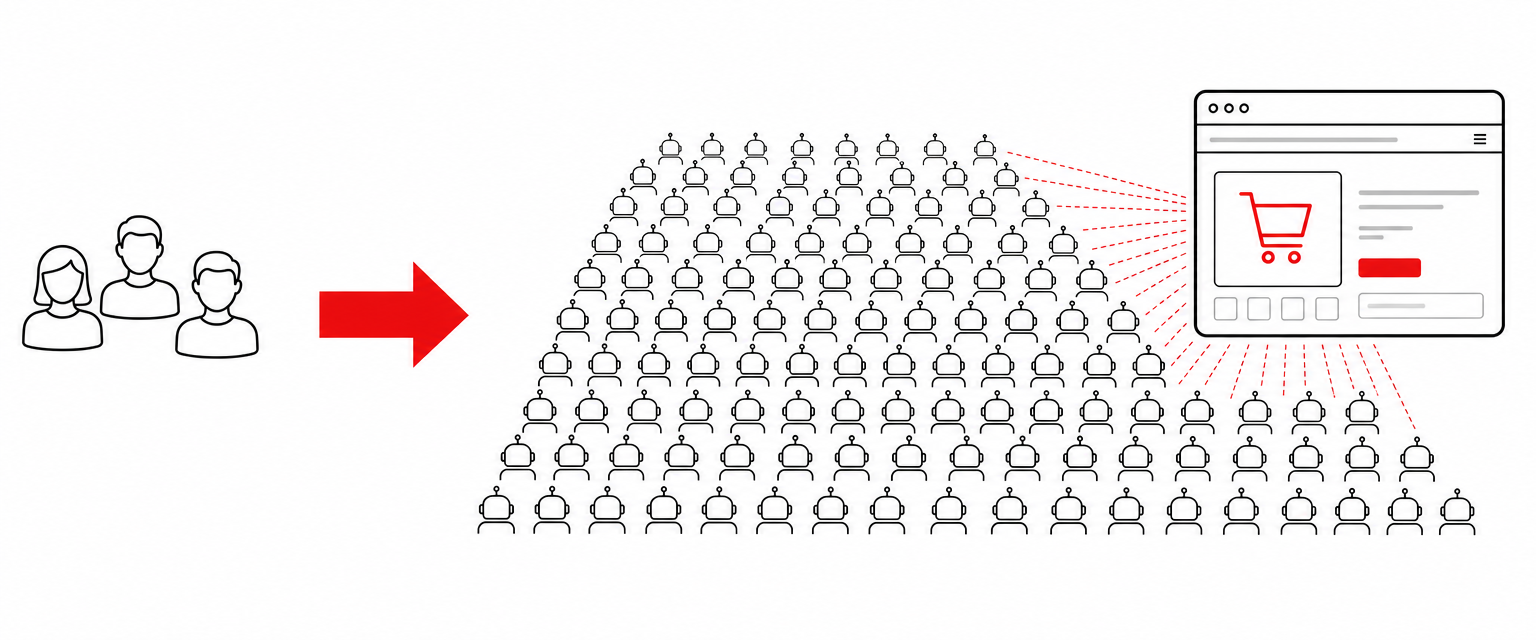
\includegraphics[width=\linewidth]{figures/agentab/scale_concept.png}
  \end{figure}
\end{frame}

% ---- What A/B testing is, and why it is heavy ----
\begin{frame}{Three Bottlenecks in A/B Testing}
  \begin{figure}[htp]
    \centering
    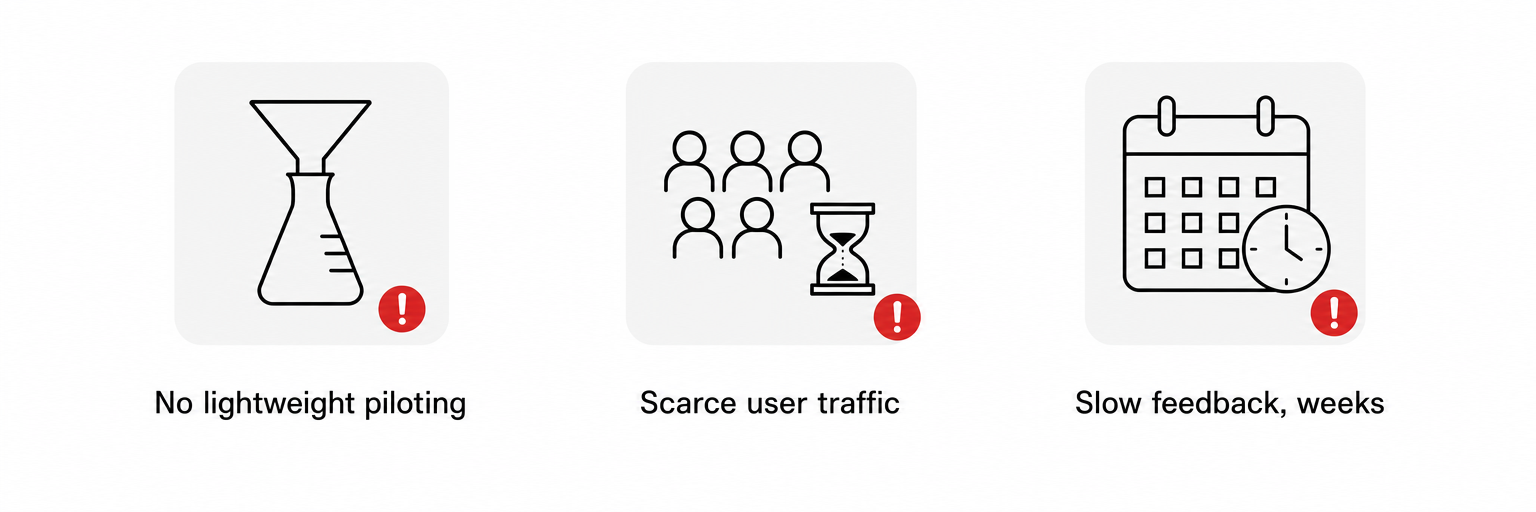
\includegraphics[width=\linewidth]{figures/agentab/bottlenecks.png}
  \end{figure}
  \centering\small From a formative study with 6 A/B-testing practitioners --- many promising ideas never get piloted before launch.
\end{frame}

% ---- The question ----
\begin{frame}[standout]
  Can we deploy \textbf{thousands} of persona-driven LLM agents on the \emph{live} website
  \vspace{6pt}

  --- to pilot an A/B test \ul{before} spending real user traffic?
\end{frame}

% ---- System overview ----
\begin{frame}{Our Solution: Agent A/B}
  \begin{figure}[htp]
    \centering
    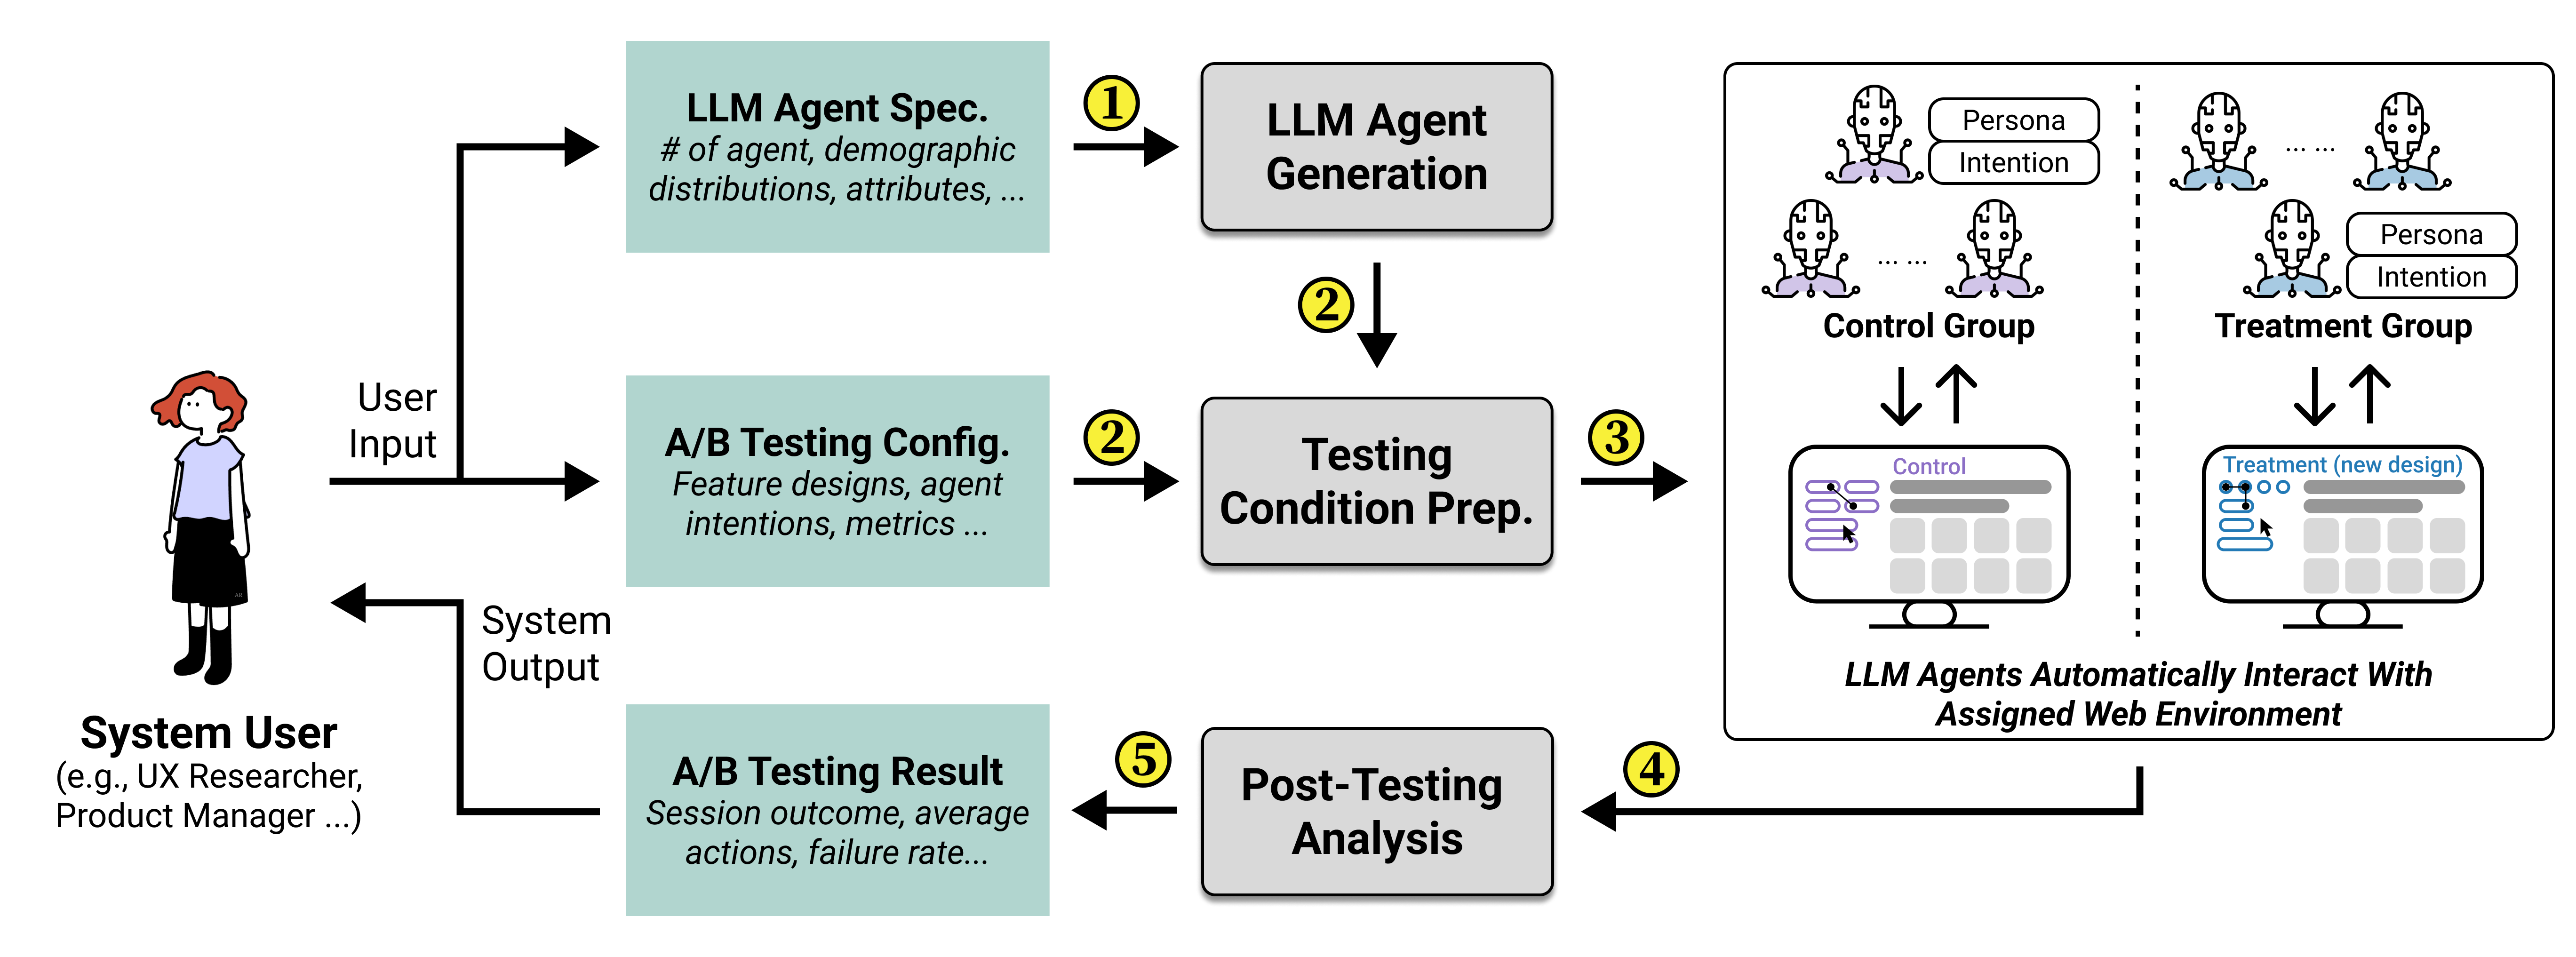
\includegraphics[width=\linewidth]{figures/agentab/abtest.png}
  \end{figure}
  \centering\small Plug-and-play with existing agent stacks (Claude computer-use, ReAct).
\end{frame}

% \begin{frame}{Inside One Agent}
%   \begin{figure}[htp]
%     \centering
%     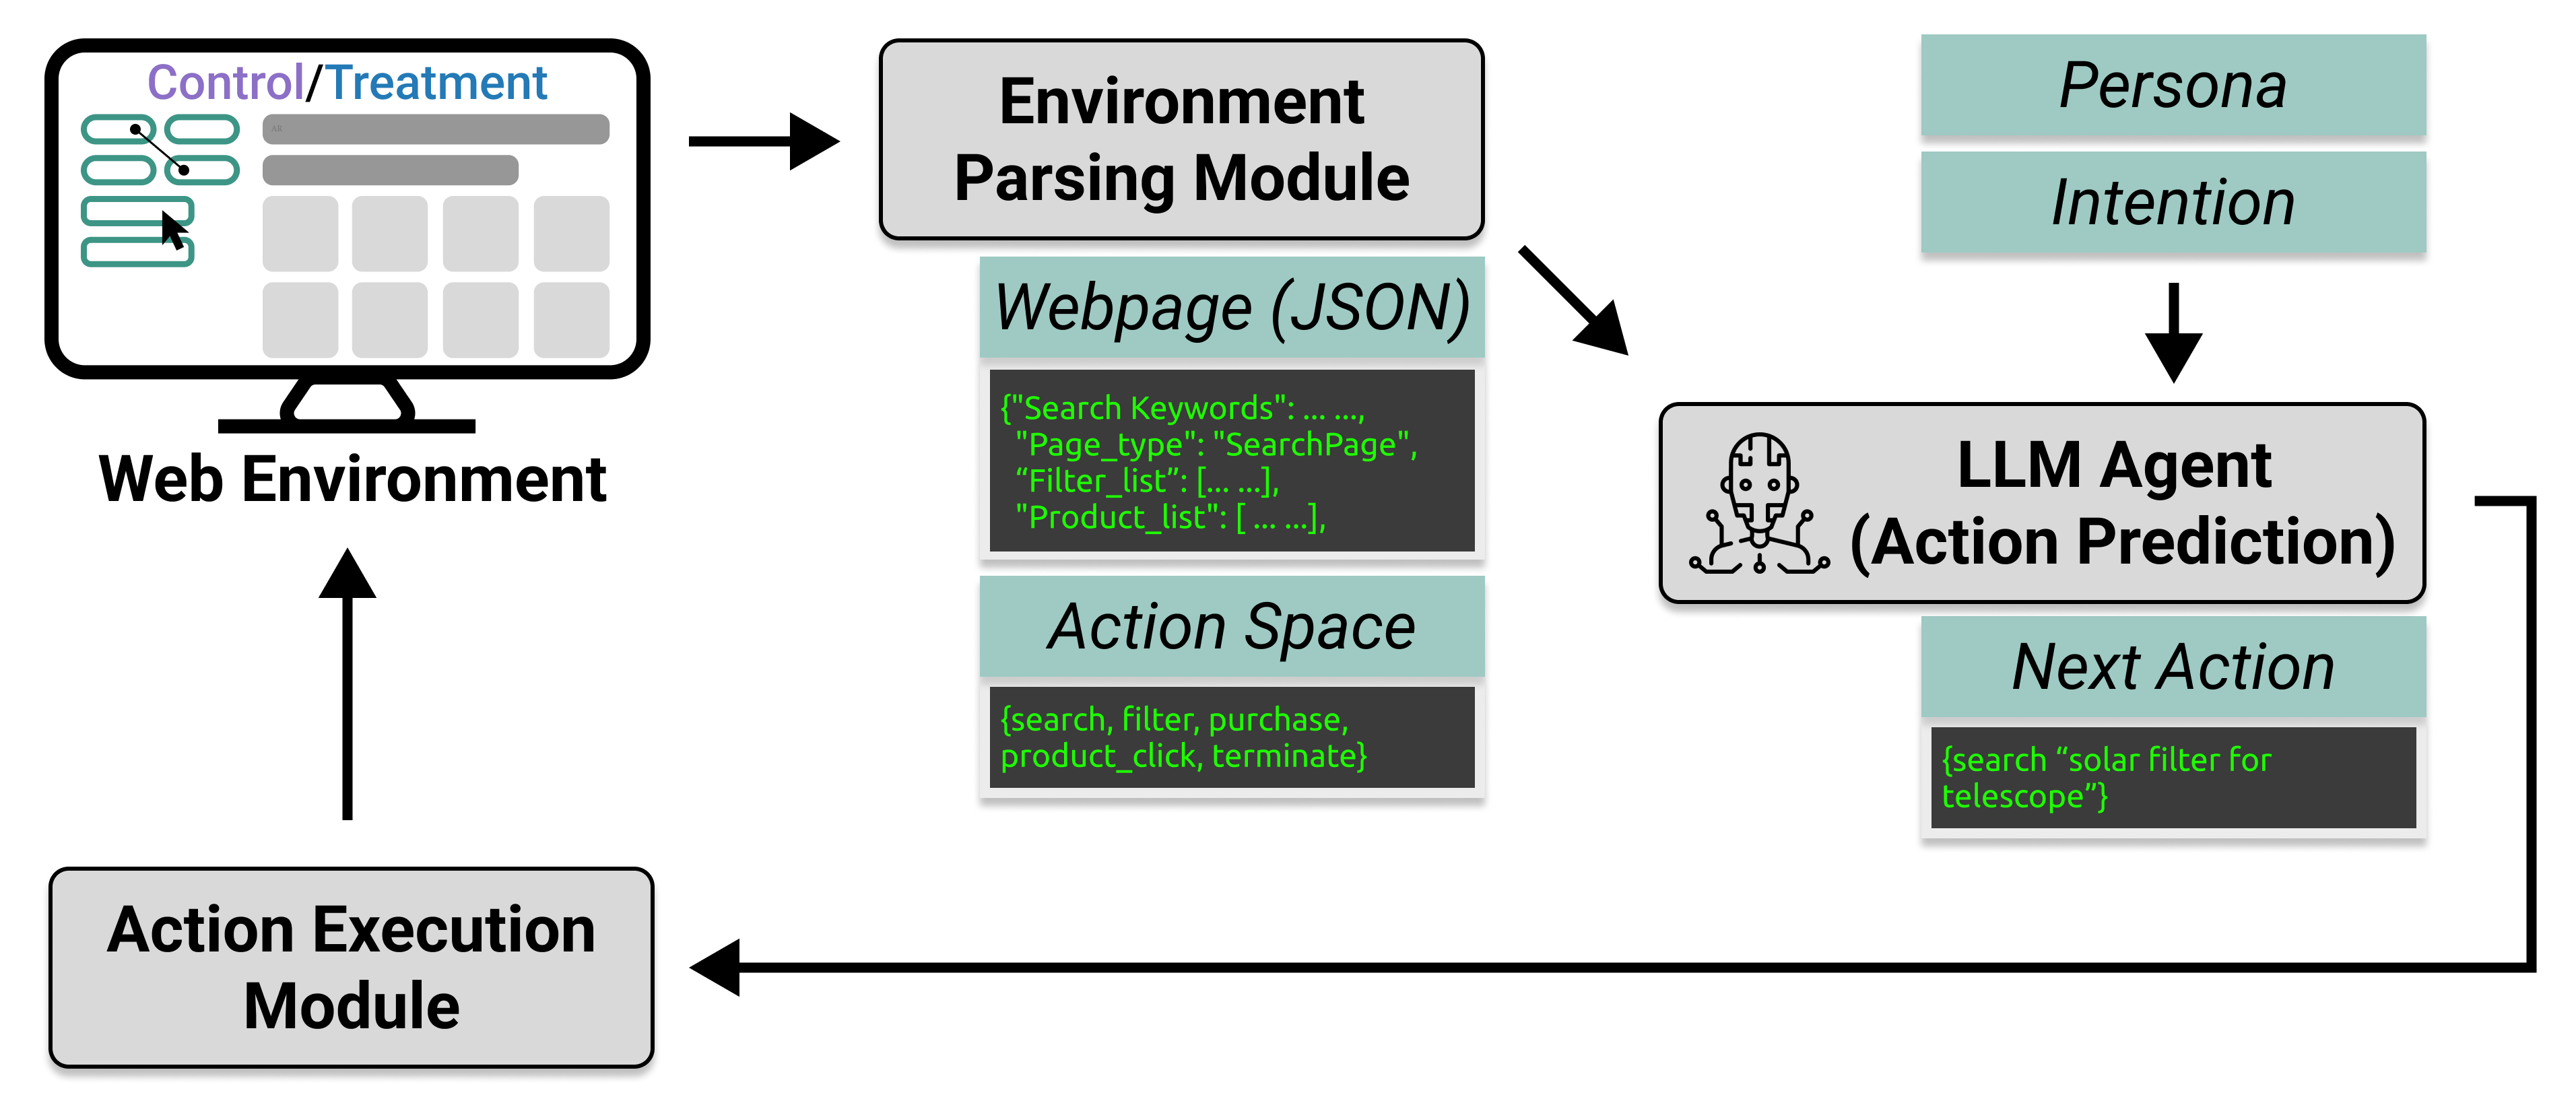
\includegraphics[width=.96\linewidth]{figures/agentab/system.png}
%   \end{figure}
% \end{frame}

% ---- Case study setup ----
\begin{frame}{Case Study: Amazon.com}
  \begin{figure}[htp]
    \centering
    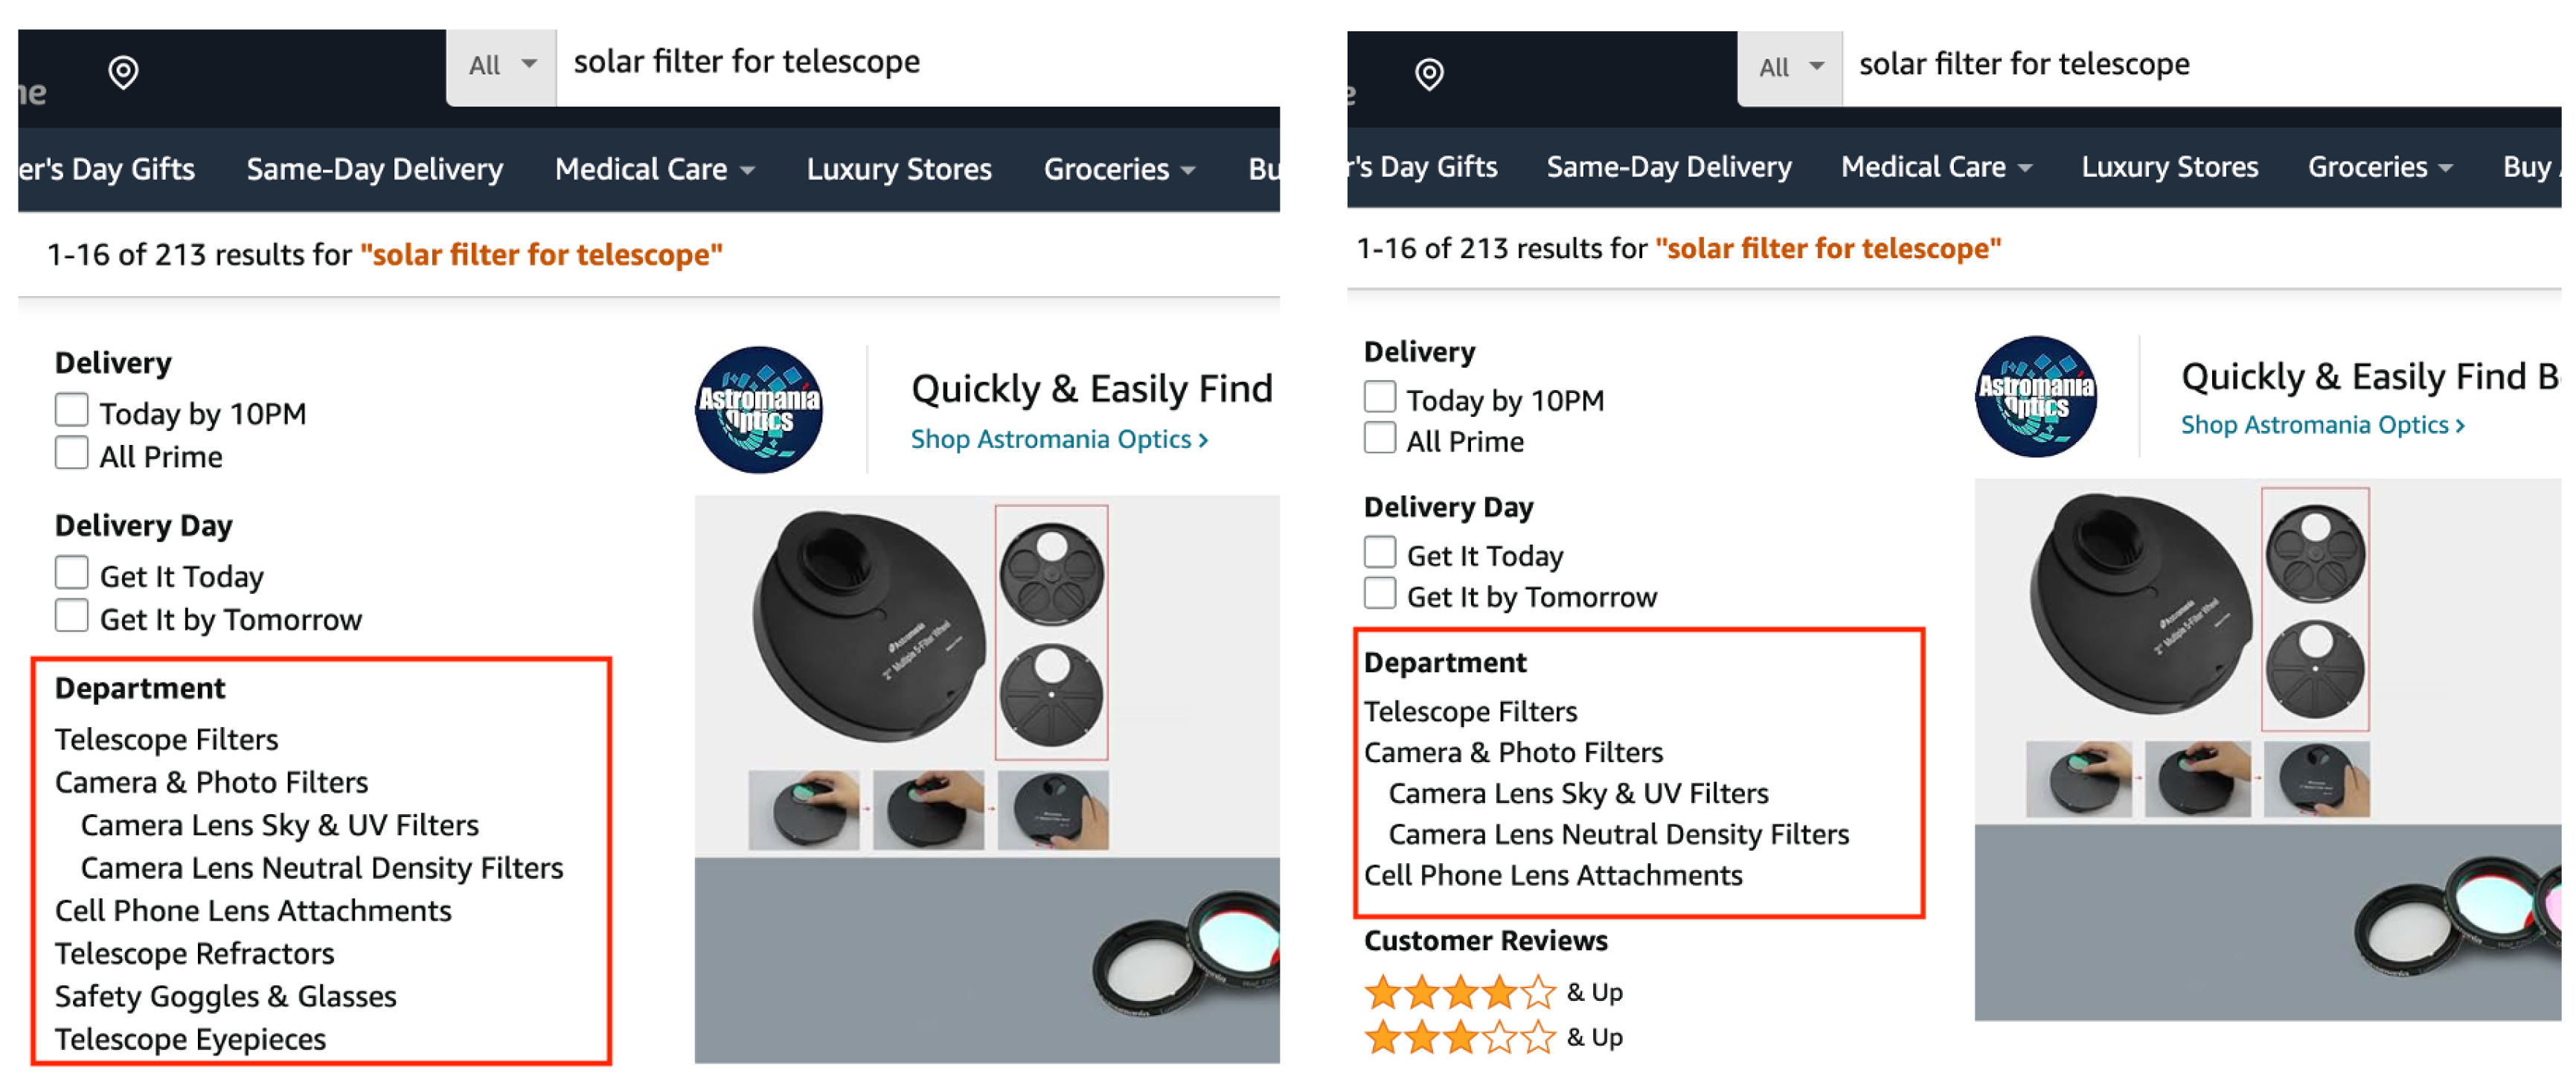
\includegraphics[width=.8\linewidth]{figures/agentab/filter_panel_design.png}
  \end{figure}
  \centering\small \textbf{Control}: full filter panel \quad vs.\quad \textbf{Treatment}: reduced panel (similarity ranking)\\
  \textbf{1,000} agents (500/condition) --- $\approx$10\% of a real A/B test.
\end{frame}

% ---- Results ----
\begin{frame}{Results: Reduced Filter $\rightarrow$ More Purchases}
  \begin{figure}[htp]
    \centering
    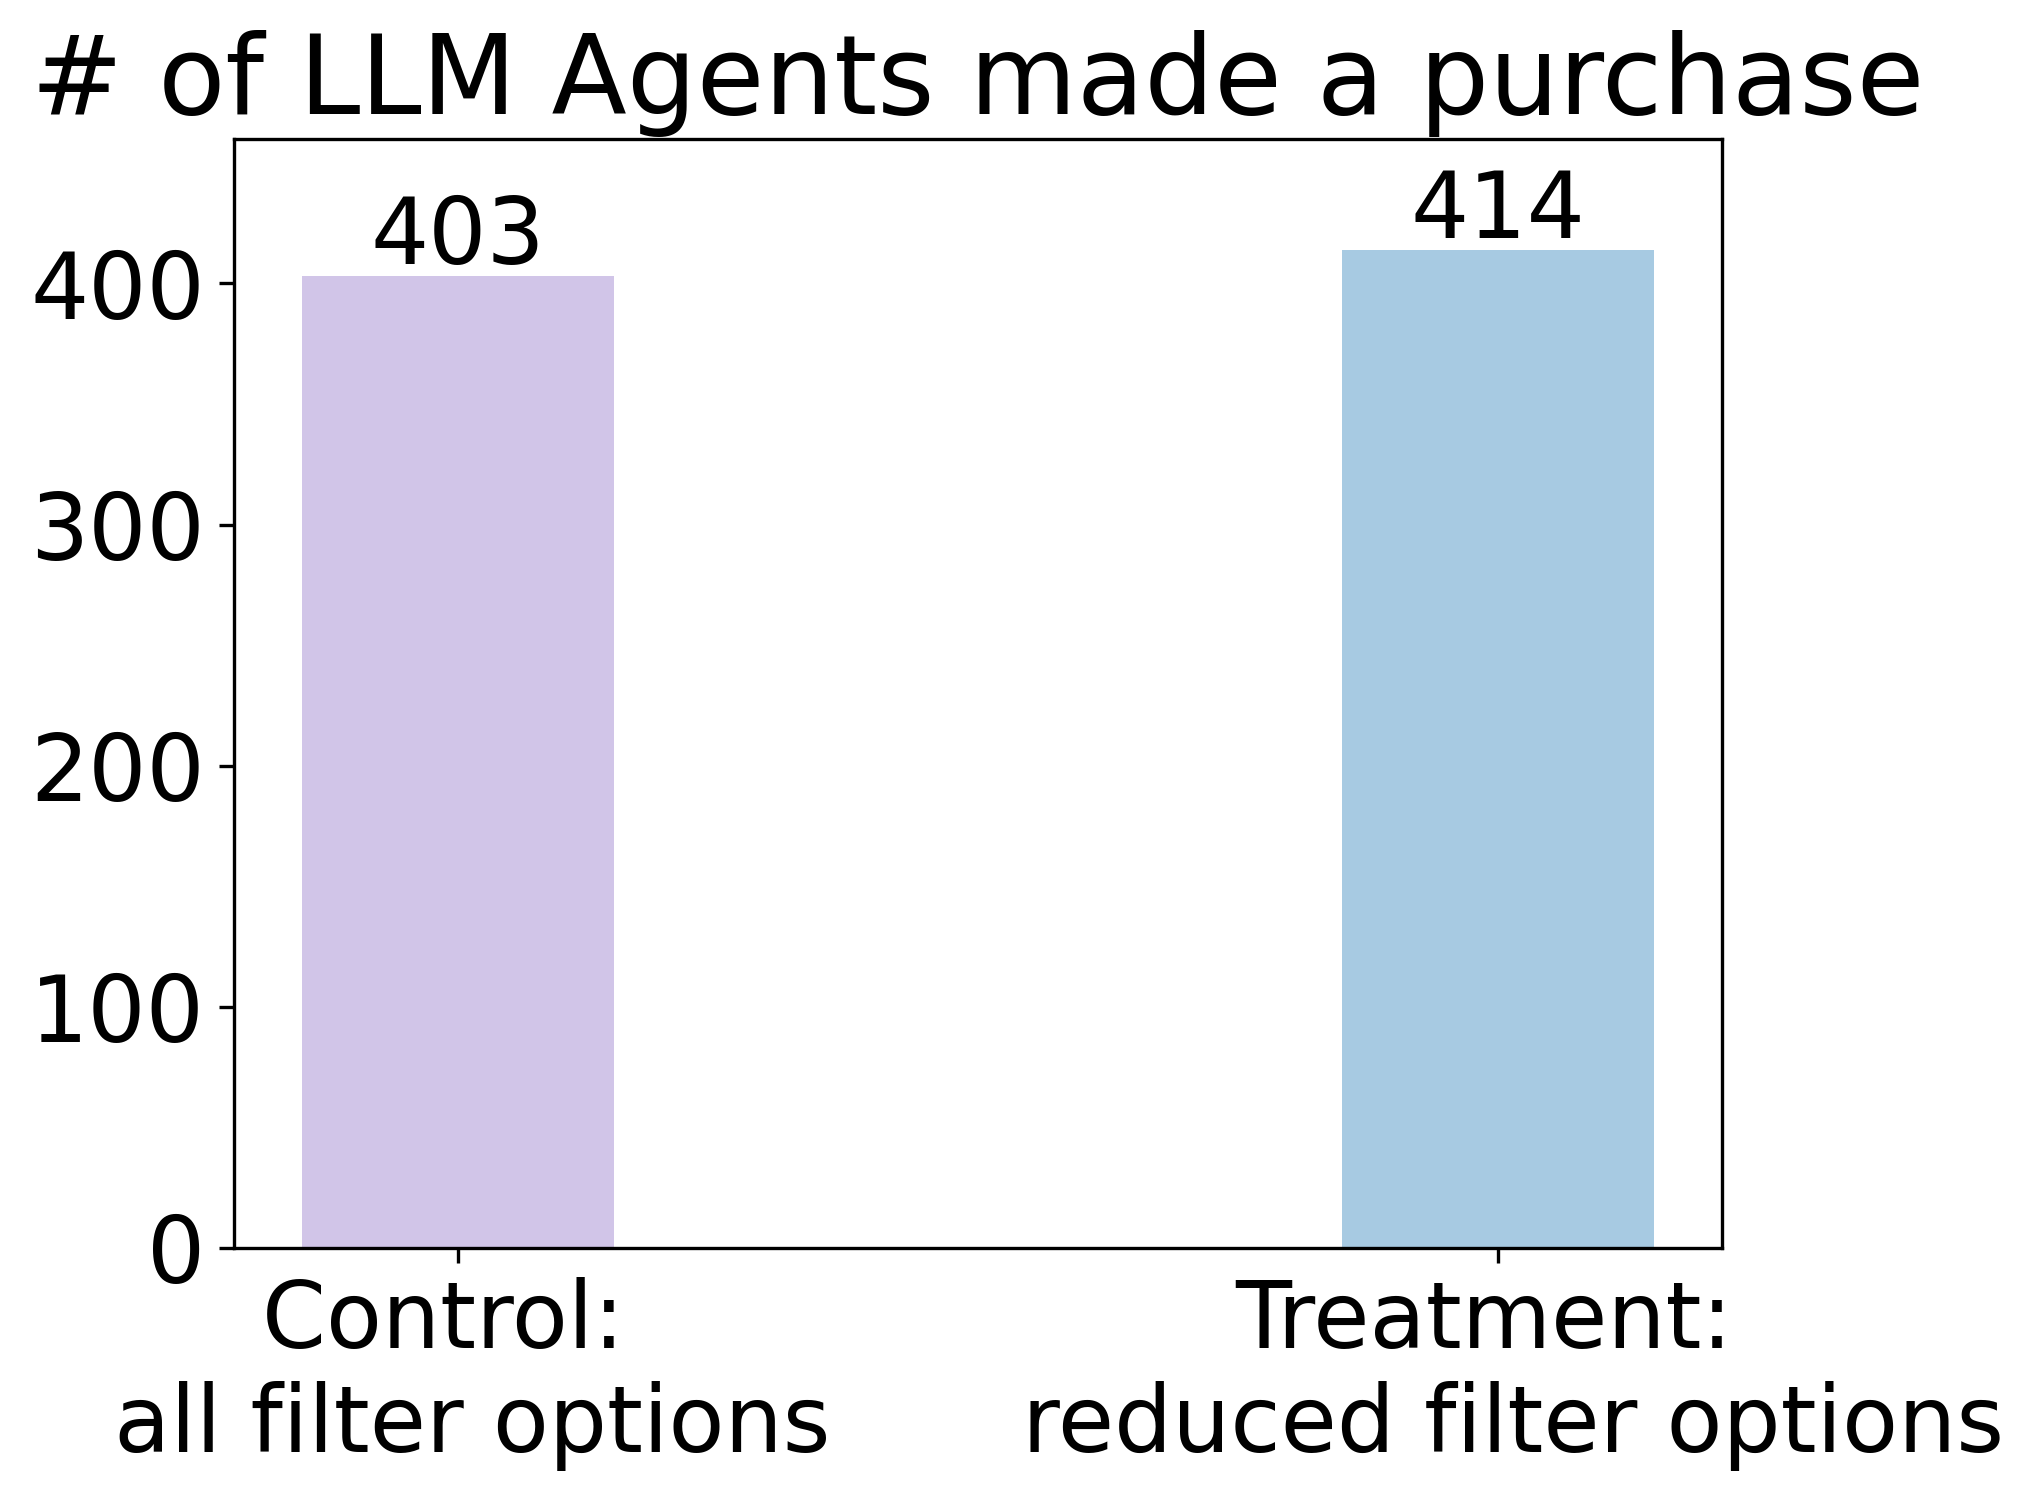
\includegraphics[width=.62\linewidth]{figures/agentab/bar.png}
  \end{figure}
  \centering\small \textbf{414 vs.\ 403} purchases --- a modest but statistically reliable increase.
\end{frame}

\begin{frame}{Subgroup Effects}
  \begin{columns}[c]
    \begin{column}{0.5\linewidth}
      \centering
      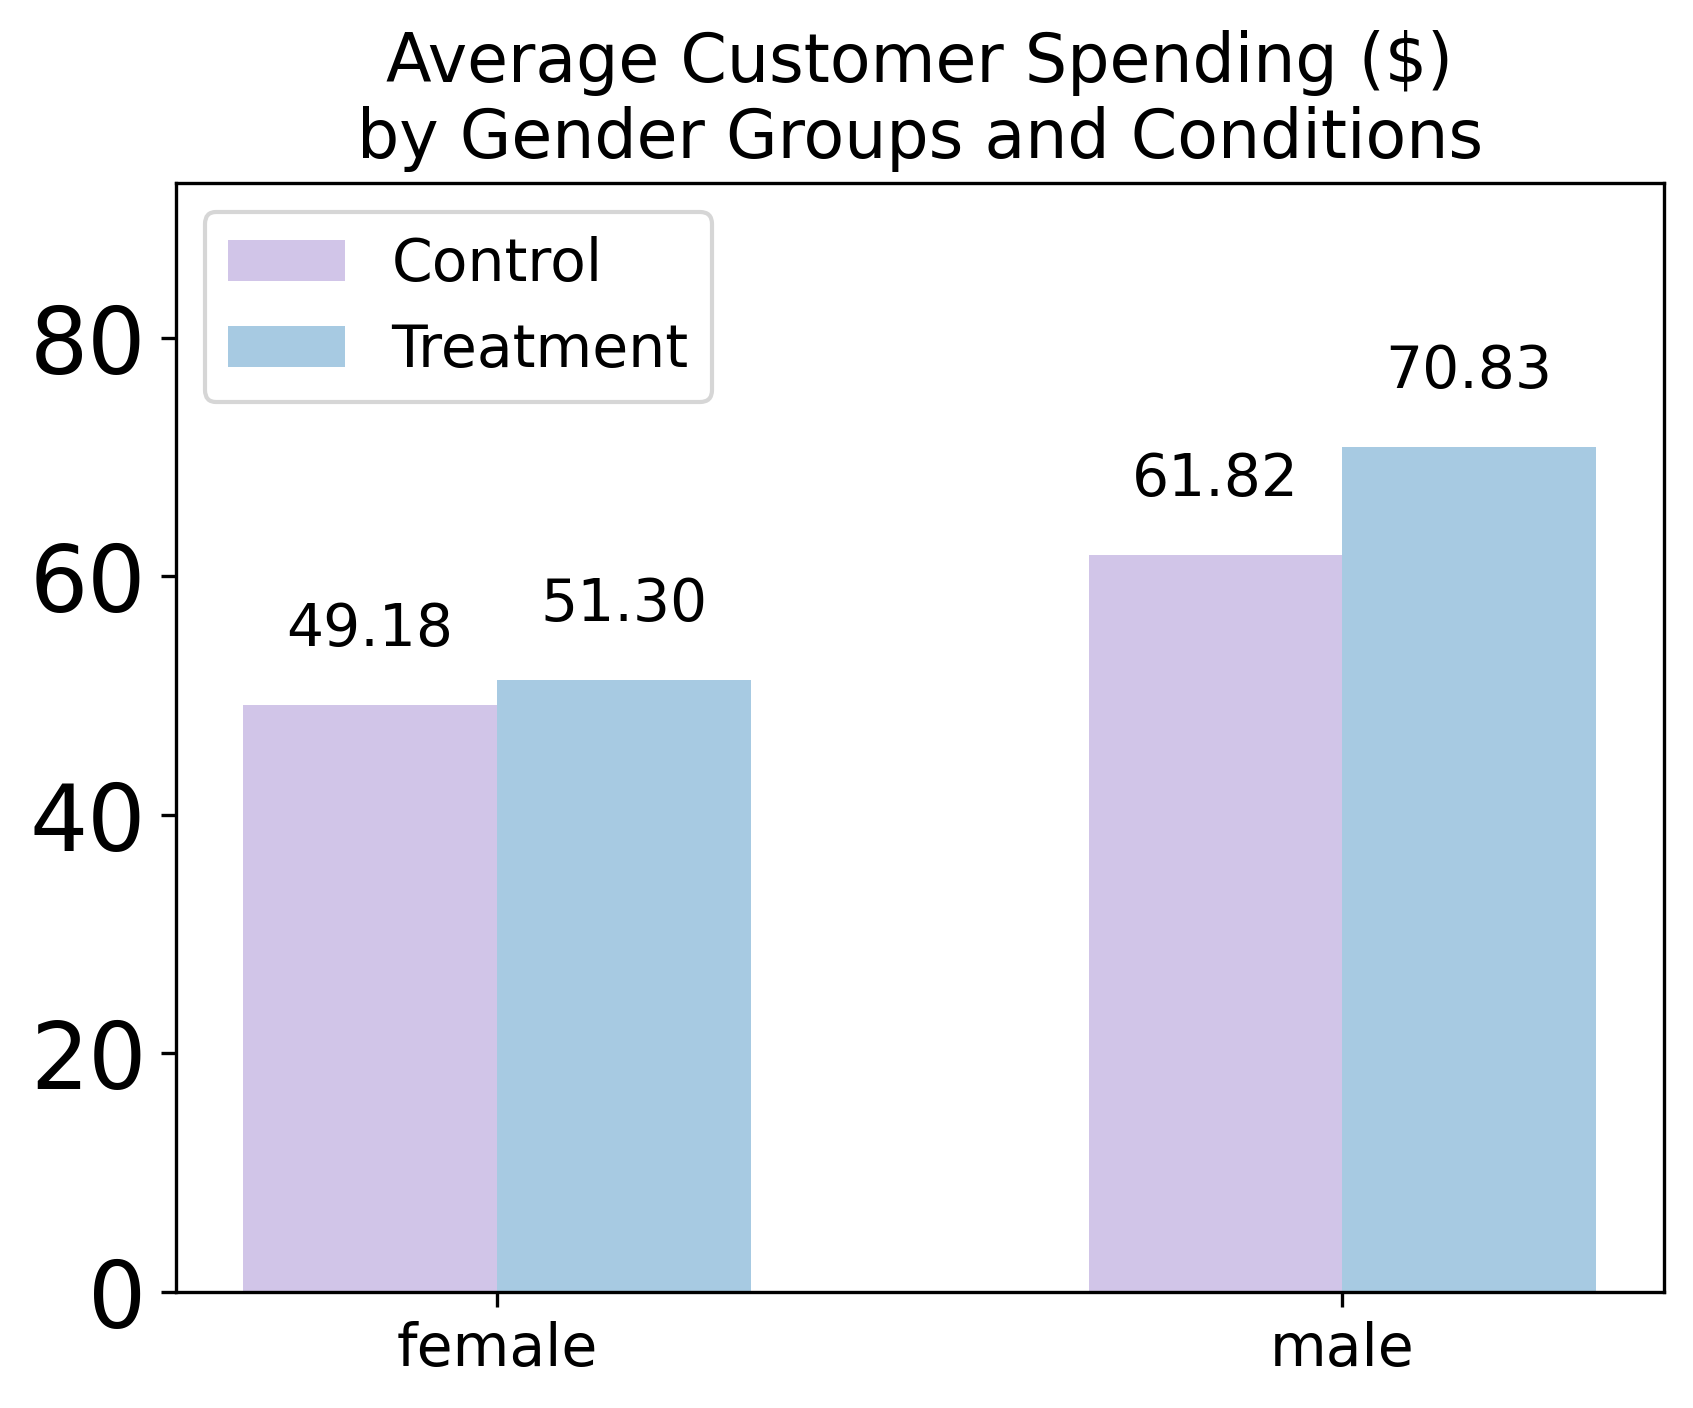
\includegraphics[width=\linewidth]{figures/agentab/control_treatment_gender_bar.png}
    \end{column}
    \begin{column}{0.5\linewidth}
      \centering
      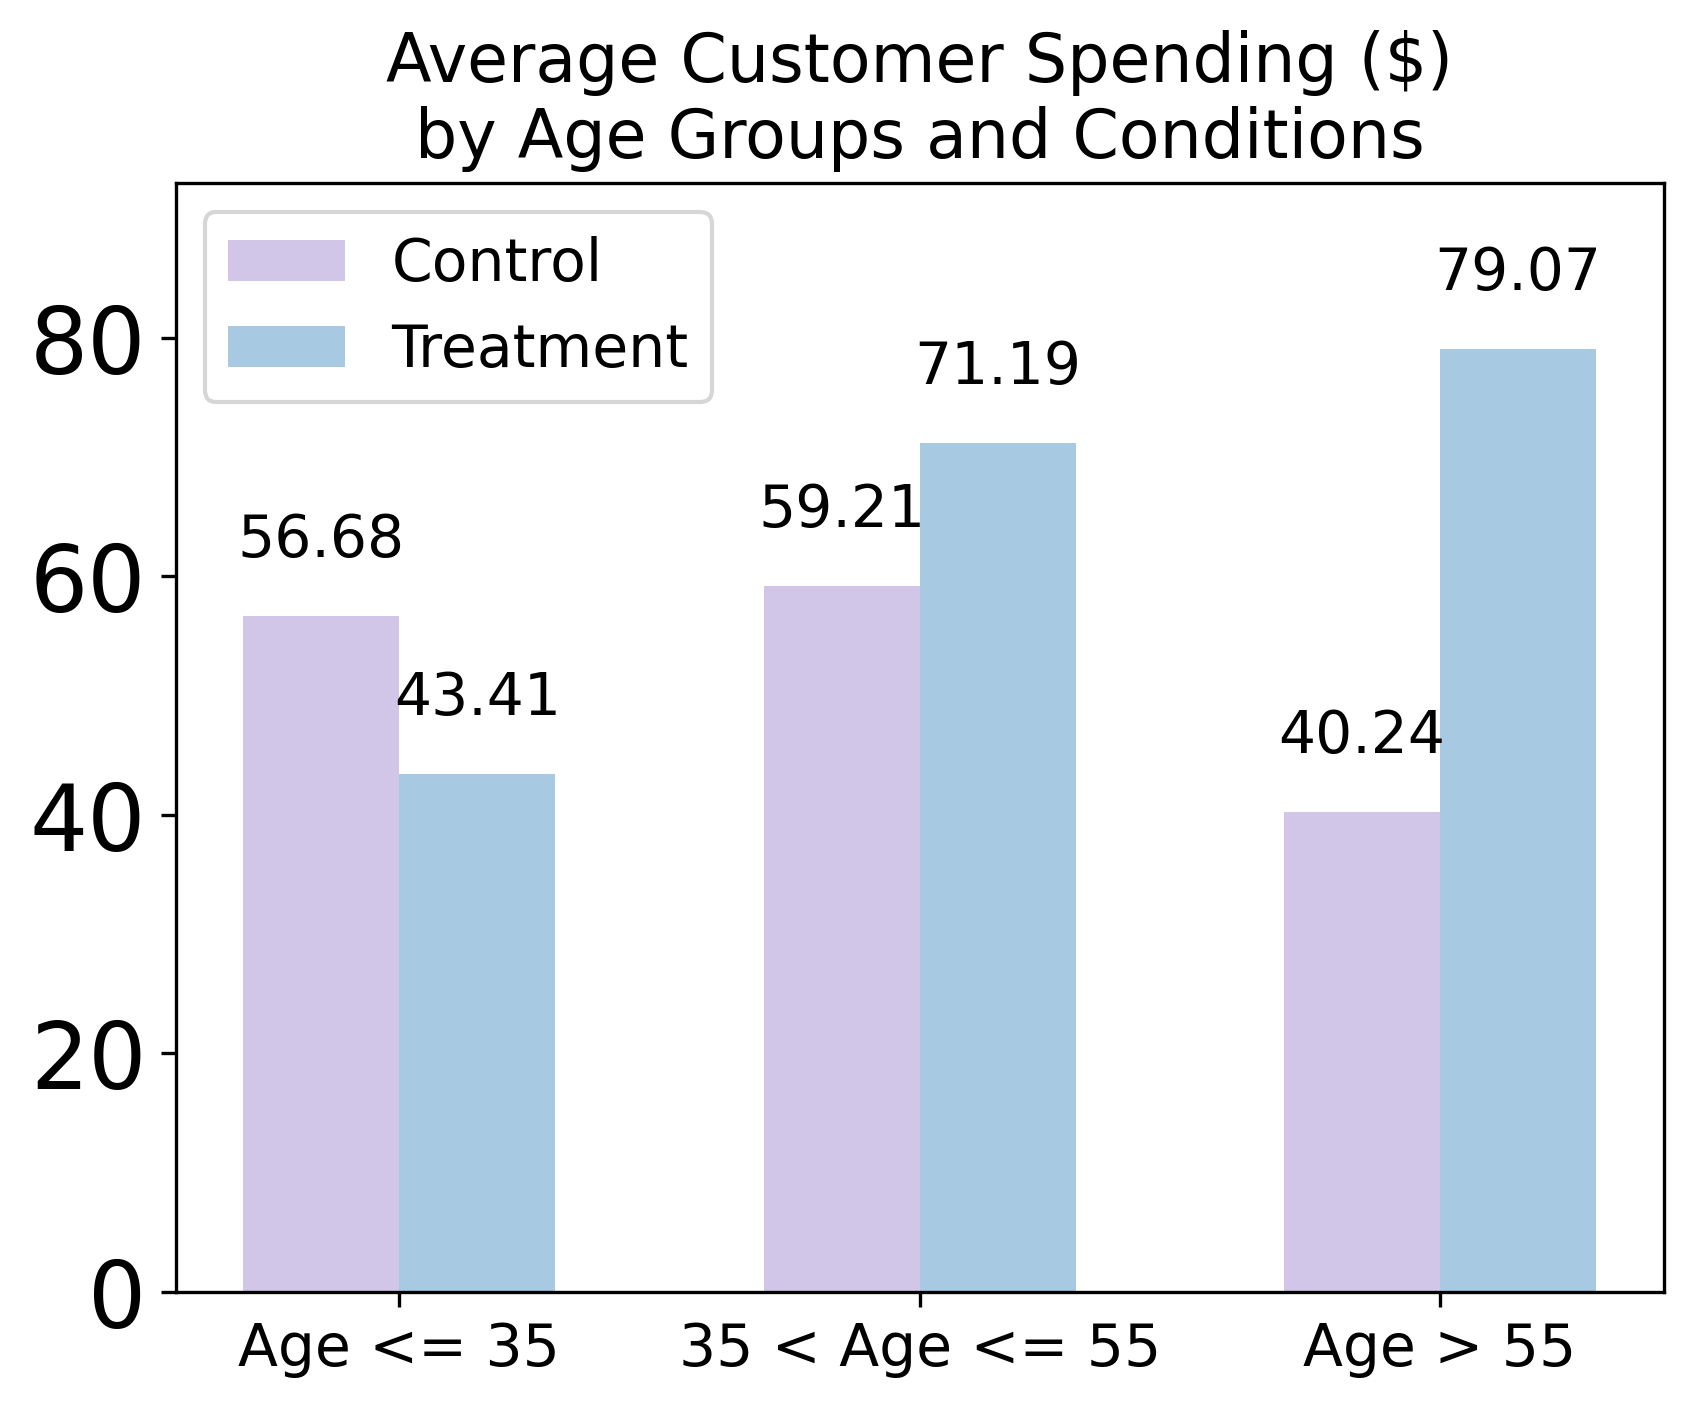
\includegraphics[width=\linewidth]{figures/agentab/control_treatment_age_bar.png}
    \end{column}
  \end{columns}
  \vspace{4pt}
  \centering\small Effects are stronger for \textbf{male} and \textbf{older} personas.
\end{frame}

% ---- Key validation ----
\begin{frame}[standout]
  Agent outcomes align \emph{directionally} with a parallel
  \textbf{large-scale human A/B experiment}.
\end{frame}

% ---- Handoff to Case Study 3 ----
\begin{frame}[standout]
  Simulated users can \ul{scale} --- \\ and point in the right direction.
  \vspace{10pt}
  \pause

  But ``directionally aligned'' $\neq$ ``accurate''.
  \vspace{4pt}

  \emph{How faithful are these agents, really?}
\end{frame}

\end{document}
